\documentclass{standalone}
\usepackage{tikz}
\usetikzlibrary{patterns, positioning}


\begin{document}
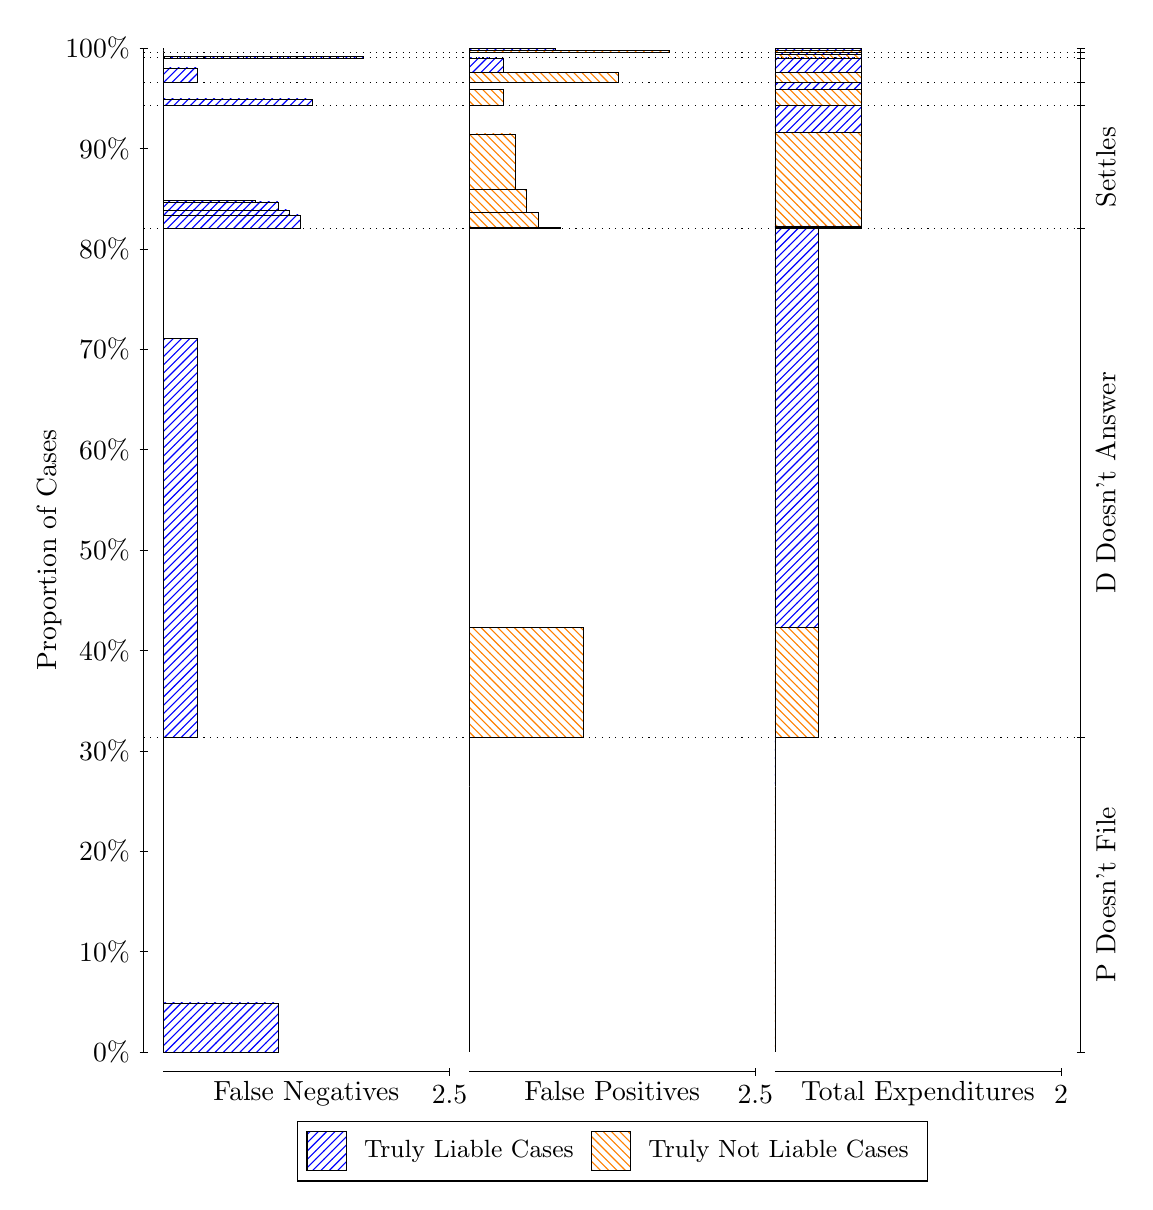
\begin{tikzpicture}
\draw[black, very thin] (1.5,1.75) -- (1.5,14.5);
\node[rotate=90, text=black, anchor=center] at (0.3, 8.125) {Proportion of Cases};
\draw[black, very thin] (1.45,1.75) -- (1.55,1.75);
\node[text=black, anchor=east] at (1.45, 1.75) {0\%};
\draw[black, very thin] (1.45,3.025) -- (1.55,3.025);
\node[text=black, anchor=east] at (1.45, 3.025) {10\%};
\draw[black, very thin] (1.45,4.3) -- (1.55,4.3);
\node[text=black, anchor=east] at (1.45, 4.3) {20\%};
\draw[black, very thin] (1.45,5.575) -- (1.55,5.575);
\node[text=black, anchor=east] at (1.45, 5.575) {30\%};
\draw[black, very thin] (1.45,6.85) -- (1.55,6.85);
\node[text=black, anchor=east] at (1.45, 6.85) {40\%};
\draw[black, very thin] (1.45,8.125) -- (1.55,8.125);
\node[text=black, anchor=east] at (1.45, 8.125) {50\%};
\draw[black, very thin] (1.45,9.4) -- (1.55,9.4);
\node[text=black, anchor=east] at (1.45, 9.4) {60\%};
\draw[black, very thin] (1.45,10.675) -- (1.55,10.675);
\node[text=black, anchor=east] at (1.45, 10.675) {70\%};
\draw[black, very thin] (1.45,11.95) -- (1.55,11.95);
\node[text=black, anchor=east] at (1.45, 11.95) {80\%};
\draw[black, very thin] (1.45,13.225) -- (1.55,13.225);
\node[text=black, anchor=east] at (1.45, 13.225) {90\%};
\draw[black, very thin] (1.45,14.5) -- (1.55,14.5);
\node[text=black, anchor=east] at (1.45, 14.5) {100\%};

\draw[black, very thin] (13.4,1.75) -- (13.4,14.5);
\draw[black, very thin] (13.35,1.75) -- (13.45,1.75);
\node[anchor=west] at (13.35, 1.75) {};
\draw[black, very thin] (13.35,5.7472) -- (13.45,5.7472);
\node[anchor=west] at (13.35, 5.7472) {};
\draw[black, very thin] (13.35,12.206) -- (13.45,12.206);
\node[anchor=west] at (13.35, 12.206) {};
\draw[black, very thin] (13.35,13.773) -- (13.45,13.773);
\node[anchor=west] at (13.35, 13.773) {};
\draw[black, very thin] (13.35,14.06) -- (13.45,14.06);
\node[anchor=west] at (13.35, 14.06) {};
\draw[black, very thin] (13.35,14.376) -- (13.45,14.376);
\node[anchor=west] at (13.35, 14.376) {};
\draw[black, very thin] (13.35,14.445) -- (13.45,14.445);
\node[anchor=west] at (13.35, 14.445) {};
\draw[black, very thin] (13.35,14.5) -- (13.45,14.5);
\node[anchor=west] at (13.35, 14.5) {};

\draw[black, very thin, pattern color=blue, pattern=north east lines] (1.75,1.75) rectangle (3.2033,2.3745);
\draw[black, very thin, pattern color=orange, pattern=north west lines] (1.75,2.3745) rectangle (1.75,5.7472);
\draw[black, very thin, pattern color=blue, pattern=north east lines] (1.75,5.7472) rectangle (2.186,10.809);
\draw[black, very thin, pattern color=orange, pattern=north west lines] (1.75,10.809) rectangle (1.75,12.206);
\draw[black, very thin, pattern color=blue, pattern=north east lines] (1.75,12.206) rectangle (3.494,12.381);
\draw[black, very thin, pattern color=blue, pattern=north east lines] (1.75,12.381) rectangle (3.3487,12.444);
\draw[black, very thin, pattern color=blue, pattern=north east lines] (1.75,12.444) rectangle (3.2033,12.545);
\draw[black, very thin, pattern color=blue, pattern=north east lines] (1.75,12.545) rectangle (2.9127,12.569);
\draw[black, very thin, pattern color=orange, pattern=north west lines] (1.75,12.569) rectangle (1.75,13.773);
\draw[black, very thin, pattern color=blue, pattern=north east lines] (1.75,13.773) rectangle (3.6393,13.855);
\draw[black, very thin, pattern color=orange, pattern=north west lines] (1.75,13.855) rectangle (1.75,14.06);
\draw[black, very thin, pattern color=blue, pattern=north east lines] (1.75,14.06) rectangle (2.186,14.247);
\draw[black, very thin, pattern color=orange, pattern=north west lines] (1.75,14.247) rectangle (1.75,14.376);
\draw[black, very thin, pattern color=blue, pattern=north east lines] (1.75,14.376) rectangle (4.2933,14.397);
\draw[black, very thin, pattern color=orange, pattern=north west lines] (1.75,14.397) rectangle (1.75,14.445);
\draw[black, very thin, pattern color=orange, pattern=north west lines] (1.75,14.445) rectangle (1.75,14.466);
\draw[black, very thin, pattern color=blue, pattern=north east lines] (1.75,14.466) rectangle (1.75,14.5);
\draw[black, very thin, pattern color=orange, pattern=north west lines] (5.6333,1.75) rectangle (5.6333,5.1227);
\draw[black, very thin, pattern color=blue, pattern=north east lines] (5.6333,5.1227) rectangle (5.6333,5.7472);
\draw[black, very thin, pattern color=orange, pattern=north west lines] (5.6333,5.7472) rectangle (7.0867,7.1433);
\draw[black, very thin, pattern color=blue, pattern=north east lines] (5.6333,7.1433) rectangle (5.6333,12.206);
\draw[black, very thin, pattern color=orange, pattern=north west lines] (5.6333,12.206) rectangle (6.796,12.218);
\draw[black, very thin, pattern color=orange, pattern=north west lines] (5.6333,12.218) rectangle (6.5053,12.408);
\draw[black, very thin, pattern color=orange, pattern=north west lines] (5.6333,12.408) rectangle (6.36,12.705);
\draw[black, very thin, pattern color=orange, pattern=north west lines] (5.6333,12.705) rectangle (6.2147,13.409);
\draw[black, very thin, pattern color=blue, pattern=north east lines] (5.6333,13.409) rectangle (5.6333,13.773);
\draw[black, very thin, pattern color=orange, pattern=north west lines] (5.6333,13.773) rectangle (6.0693,13.977);
\draw[black, very thin, pattern color=blue, pattern=north east lines] (5.6333,13.977) rectangle (5.6333,14.06);
\draw[black, very thin, pattern color=orange, pattern=north west lines] (5.6333,14.06) rectangle (7.5227,14.189);
\draw[black, very thin, pattern color=blue, pattern=north east lines] (5.6333,14.189) rectangle (6.0693,14.376);
\draw[black, very thin, pattern color=orange, pattern=north west lines] (5.6333,14.376) rectangle (5.6333,14.424);
\draw[black, very thin, pattern color=blue, pattern=north east lines] (5.6333,14.424) rectangle (5.6333,14.445);
\draw[black, very thin, pattern color=orange, pattern=north west lines] (5.6333,14.445) rectangle (8.1767,14.466);
\draw[black, very thin, pattern color=blue, pattern=north east lines] (5.6333,14.466) rectangle (6.7233,14.5);
\draw[black, very thin, pattern color=orange, pattern=north west lines] (9.5167,1.75) rectangle (9.5167,5.1227);
\draw[black, very thin, pattern color=blue, pattern=north east lines] (9.5167,5.1227) rectangle (9.5167,5.7472);
\draw[black, very thin, pattern color=orange, pattern=north west lines] (9.5167,5.7472) rectangle (10.062,7.1433);
\draw[black, very thin, pattern color=blue, pattern=north east lines] (9.5167,7.1433) rectangle (10.062,12.206);
\draw[black, very thin, pattern color=orange, pattern=north west lines] (9.5167,12.206) rectangle (10.607,12.218);
\draw[black, very thin, pattern color=blue, pattern=north east lines] (9.5167,12.218) rectangle (10.607,12.242);
\draw[black, very thin, pattern color=orange, pattern=north west lines] (9.5167,12.242) rectangle (10.607,13.433);
\draw[black, very thin, pattern color=blue, pattern=north east lines] (9.5167,13.433) rectangle (10.607,13.773);
\draw[black, very thin, pattern color=orange, pattern=north west lines] (9.5167,13.773) rectangle (10.607,13.977);
\draw[black, very thin, pattern color=blue, pattern=north east lines] (9.5167,13.977) rectangle (10.607,14.06);
\draw[black, very thin, pattern color=orange, pattern=north west lines] (9.5167,14.06) rectangle (10.607,14.189);
\draw[black, very thin, pattern color=blue, pattern=north east lines] (9.5167,14.189) rectangle (10.607,14.376);
\draw[black, very thin, pattern color=orange, pattern=north west lines] (9.5167,14.376) rectangle (10.607,14.424);
\draw[black, very thin, pattern color=blue, pattern=north east lines] (9.5167,14.424) rectangle (10.607,14.445);
\draw[black, very thin, pattern color=orange, pattern=north west lines] (9.5167,14.445) rectangle (10.607,14.466);
\draw[black, very thin, pattern color=blue, pattern=north east lines] (9.5167,14.466) rectangle (10.607,14.5);
\draw[black, dotted] (1.5,5.7472) -- (13.4,5.7472);
\draw[black, dotted] (1.5,12.206) -- (13.4,12.206);
\draw[black, dotted] (1.5,13.773) -- (13.4,13.773);
\draw[black, dotted] (1.5,14.06) -- (13.4,14.06);
\draw[black, dotted] (1.5,14.376) -- (13.4,14.376);
\draw[black, dotted] (1.5,14.445) -- (13.4,14.445);
\draw[black, very thin] (1.75,1.5) -- (5.3833,1.5);
\node[text=black, anchor=north] at (3.5667, 1.5) {False Negatives};
\draw[black, very thin] (5.3833,1.45) -- (5.3833,1.55);
\node[text=black, anchor=north] at (5.3833, 1.45) {2.5};

\draw[black, very thin] (5.6333,1.5) -- (9.2667,1.5);
\node[text=black, anchor=north] at (7.45, 1.5) {False Positives};
\draw[black, very thin] (9.2667,1.45) -- (9.2667,1.55);
\node[text=black, anchor=north] at (9.2667, 1.45) {2.5};

\draw[black, very thin] (9.5167,1.5) -- (13.15,1.5);
\node[text=black, anchor=north] at (11.333, 1.5) {Total Expenditures};
\draw[black, very thin] (13.15,1.45) -- (13.15,1.55);
\node[text=black, anchor=north] at (13.15, 1.45) {2};

\node[text=black, centered, rotate=90] at (13.72, 3.7486) {P Doesn't File};
\node[text=black, centered, rotate=90] at (13.72, 8.9764) {D Doesn't Answer};
\node[text=black, centered, rotate=90] at (13.72, 12.989) {Settles};





\draw (7.449999999999999,1.5) node[draw=none] (baseCoordinate) {};
\begin{scope}[align=center]
        \matrix[scale=0.5, draw=black, below=0.5cm of baseCoordinate, nodes={draw}, column sep=0.1cm]{
            \node[rectangle, draw, minimum width=0.5cm, minimum height=0.5cm, pattern color=blue, pattern=north east lines] {}; &
            \node[draw=none, font=\small, text=black] (B) {Truly Liable Cases}; &
            \node[rectangle, draw, minimum width=0.5cm, minimum height=0.5cm, pattern color=orange, pattern=north west lines] {}; &
            \node[draw=none, font=\small, text=black] (B) {Truly Not Liable Cases}; \\
            };
\end{scope}

\end{tikzpicture}
\end{document}